% Metódy inžinierskej práce

\documentclass[10pt,twoside,slovak,a4paper]{article}

\usepackage[slovak]{babel}

\usepackage[IL2]{fontenc} 
\usepackage[utf8]{inputenc}
\usepackage{graphicx}
\usepackage{url} 
\usepackage{hyperref} 

\usepackage{cite}



\title{{\bf Modelovanie spracovania elektronického podania ÚPVS sekvenčnými UML diagramami}\thanks{Semestrálny projekt v predmete Metódy inžinierskej práce, ak. rok 2021/22, vedenie: Vladimír Mlynarovič}}

\author{Viktor Uhlár\\[2pt]
	{\small Slovenská technická univerzita v Bratislave}\\
	{\small Fakulta informatiky a informačných technológií}\\
	{\small \texttt{xuhlar@stuba.sk}}
	}

\date{\small 6. november 2021} 


\linespread{1.3}
\begin{document}



\begin {titlepage}
\centering
\maketitle

\begin{abstract}


\noindent{Ústredný portál verejnej správy (ÚPVS) je centrálnym miestom na podávanie a spracovanie elektronických podaní. Pre agendové informačné systémy poskytuje možnosť integrácie tak, aby bolo možné zasielať elektronické podania priamo z vlastných informačných systémov (teda bez nutosti priuhlasovania sa do elektronických schránok pomocou eID - elektronického občianskeho preukazu).}\newline
\noindent{Keďže postupnosť spracovania elektronického podania závisí od jeho účelu, musí byť pred fázou samotnej integrácie vypracovaný model ``workflow“. ÚPVS pre tento účel vyžaduje tzv. Dohodu o integračnom zámere, kde je spracovanie modelované vo forme sekvenčného UML diagramu.
V tejto práci sa teda budem venovať teórii modelovania sekvenčných UML modelov s konrétnym príkladom pre spracovanie elektronického rozhodnutia ``fiktívneho“  OVM (orgánu verejnej moci SR).}

\end{abstract}

\end{titlepage}
\flushleft
\section{Úvod}\label{1sek}

Ústredný portál verejnej správy (ÚPVS) je centrálnym miestom na podávanie a spracovanie elektronických podaní. Pre agendové informačné systémy poskytuje možnosť integrácie tak, aby bolo možné pristupovať k elektronickej schránke priamo z vlastných informačných systémov - teda bez nutosti prihlasovania sa eID - elektronického občianskeho preukazu.\\

Keďže spôsob pripojenia môže byť rôzny, správca ÚPVS (Národná agentúra pre sieťové a elektronické služby - NASES) vyžaduje podrobný integračný zámer, ktorého súčasťou je aj modelovanie integrácie vo fornme sekvenčného UML diagramu.\newline

V tejto práci sa teda budem venovať:

\begin{itemize}
\item Rámcovému popisu UML a typov diagramov
\item Spôsobu tvorby sekvenčných UML diagramov
\item Jednoduchému nástroju pre modelovanie UML diagramov
\item Modelovej integračnej situácie pripojenia na ÚPVS a popisu tvorby súvisiaceho sekvenčného UML diagramu
\end{itemize}

Informácie pre vytvorenie tejto práce som čerpal:

\begin{itemize}
\item Z integračnej dokumentácie spoločnosti NASES
\item Z internetových zdrojov ku UML modelovaniu
\item Z praktickej skúsenosti pri spolupráci v rámci integračného ÚPVS projektu
\end{itemize}
Zoznam konkrétnej použitej literatúry je uvedený v prílohe Literatúra.\\

Práca môže byť užitočná nielen pre analytikov, ktorí zodpovedajú za modelovanie integračných ``ÚPVS“ projektov, ale aj pre všeobecnejšie pochopenie zmyslu sekvenčných diagramov (ako integrálnej súčasti software development cyklov).


\section{Popis UML a rozdelenie typov diagramov} \label{2sek}

UML znamená Unified Modeling Language, teda grafický jazyk na vizualizáciu, špecifikáciu, navrhovanie a dokumentáciu programových systémov. 
\newpage
UML ponúka štandardný spôsob zápisu tak návrhov systémov vrátane konceptuálnych prvkov ako sú business procesy a systémové funkcie, tak konkrétnych prvkov ako sú príkazy programovacieho jazyka, databázové schémy a znovupoužiteľné programové komponenty.\cite{WIKI}\newline

Pomocou UML je možné modelovať niekoľko rozličných diagramov. Ich charakteristika je zrejmá z nasledovného obrázku\cite{UMLUni}:


\begin{figure}[h]
\centering
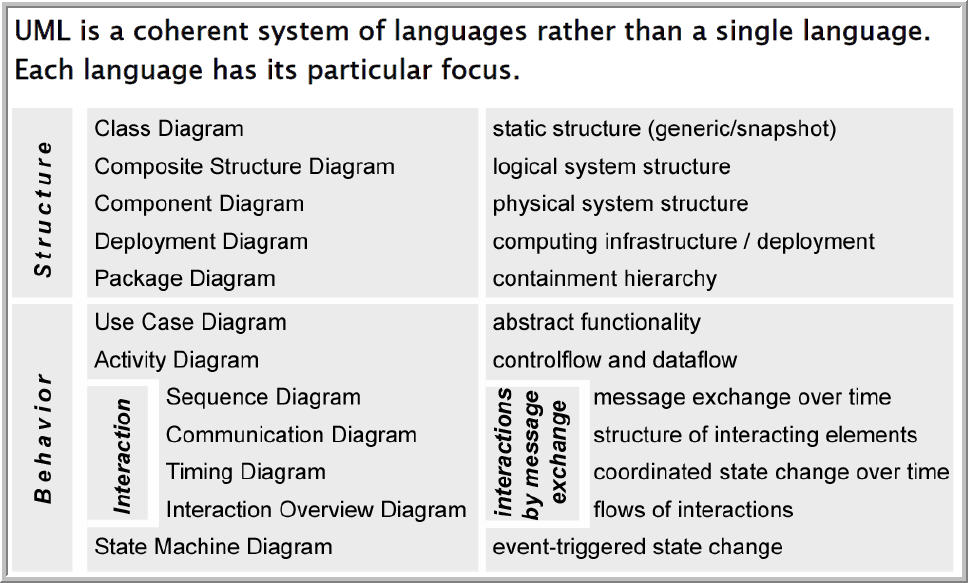
\includegraphics[width=\textwidth]{Images/Obr1.jpg}
\end{figure}

 Diagramy je teda možné rozdeliť do 3 základných skupín\cite{WIKI}:

\begin{enumerate}
\item Štruktúrne diagramy, kam patria:
	\begin{itemize}
	\item diagram tried (class diagram)
	\item diagram komponentov (component diagram)
	\item diagram zloženej štruktúry (composite structure diagram)
	\item diagram nasadenia (deployment diagram)
	\item diagram balíčkov (package diagram)
	\item diagram objektov (object diagram), nazýva sa aj diagram inštancií
	\end{itemize}
\item Diagramy správania, kam patria:
	\begin{itemize}
	\item diagram aktivít (activity diagram)
	\item diagram prípadov použitia (use case diagram)
	\item stavový diagram (state machine diagram)
	\end{itemize}
\newpage
\item Diagramy interakcie, kam patria:
	\begin{itemize}
	\item sekvenčný diagram (sequence diagram)
	\item diagram komunikácie (communication diagram) - predtým diagram spolupráce (collaboration diagram)
	\item diagram prehľadu interakcií (interaction overview diagram)
	\item diagram časovania (timing diagram)
	\end{itemize}
\end{enumerate}



\section{Sekvenčný diagram a jeho modelovanie} \label{3sek}

Skevenčný diagram modeluje interakciu medzi objektami počas konkrétneho ``use case“, teda prípadu použitia. Graficky ilustruje, ako rozličné časti systému navzájom spolupracujú tak, aby zrealizovali požadovanú funkciu. Zjednodušene povedané: sekvenčný diagram ukazuje postup činností rozličných častí systému\cite{SDT}.\newline

Pri zobrazení sa využívanie niekoľko značiek, pričom k najpoužívanejším patria:
\begin{itemize}
	\item Lifeline – životná línia
	\item Actor – účinkujúci
	\item Activity – aktivita
	\item State – stav
	\item Message arrow –tok informácie, ktorý môže byť:
		\begin{itemize}
		\item Synchronous (synchrónna)
		\item Asynchronous (nesynchrónna)
		\end{itemize}
\end{itemize}

Na nasledovnom obrázku je ilustrácia jednoduchého sekvenčného diagramu, využívajúceho vyššie uvedené značky\cite{SDT}:
\begin{figure}[h]
\centering
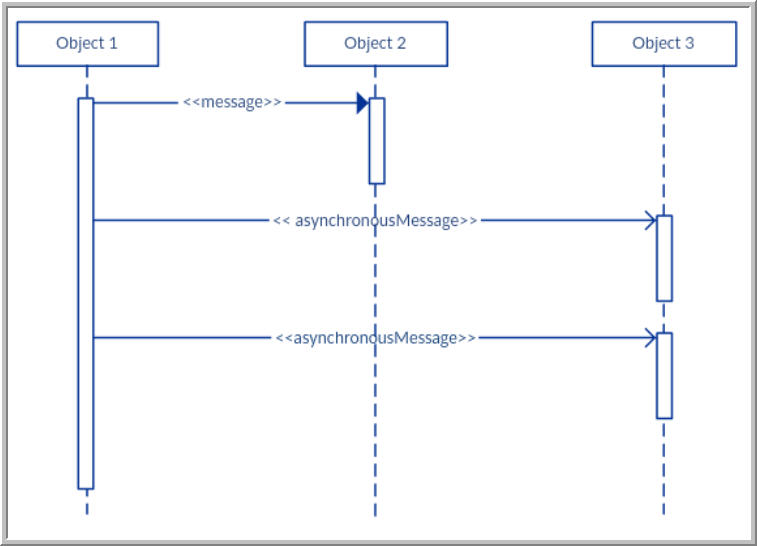
\includegraphics[width=\textwidth]{Images/Obr2.jpg}
\end{figure}


\newpage
\section{Nástroj na modelovanie formou sekvenčného UML diagramu} \label{4sek}

..... nástroj bude doplnený...

\section{Integračný scenár a jeho modelovanie} \label{5sek}

..... test a diagramy budú doplnené... \\



\section{Zhodnotenie} \label{6sek} 
..... zhodnotenie bude doplnené... \\



\bibliography{Uhlar_Literatura}
\bibliographystyle{abbrv} 
\end{document}
